\chapter{Coordination Protocol}
\kim

\noindent
This chapter describes the protocol the client has to follow when using the TravelGood service. We have illustrated this protocol with a UML state machine diagram. This state machine can be seen in Fig.~\ref{fig:protocol}.

\begin{figure}[H]
\centering
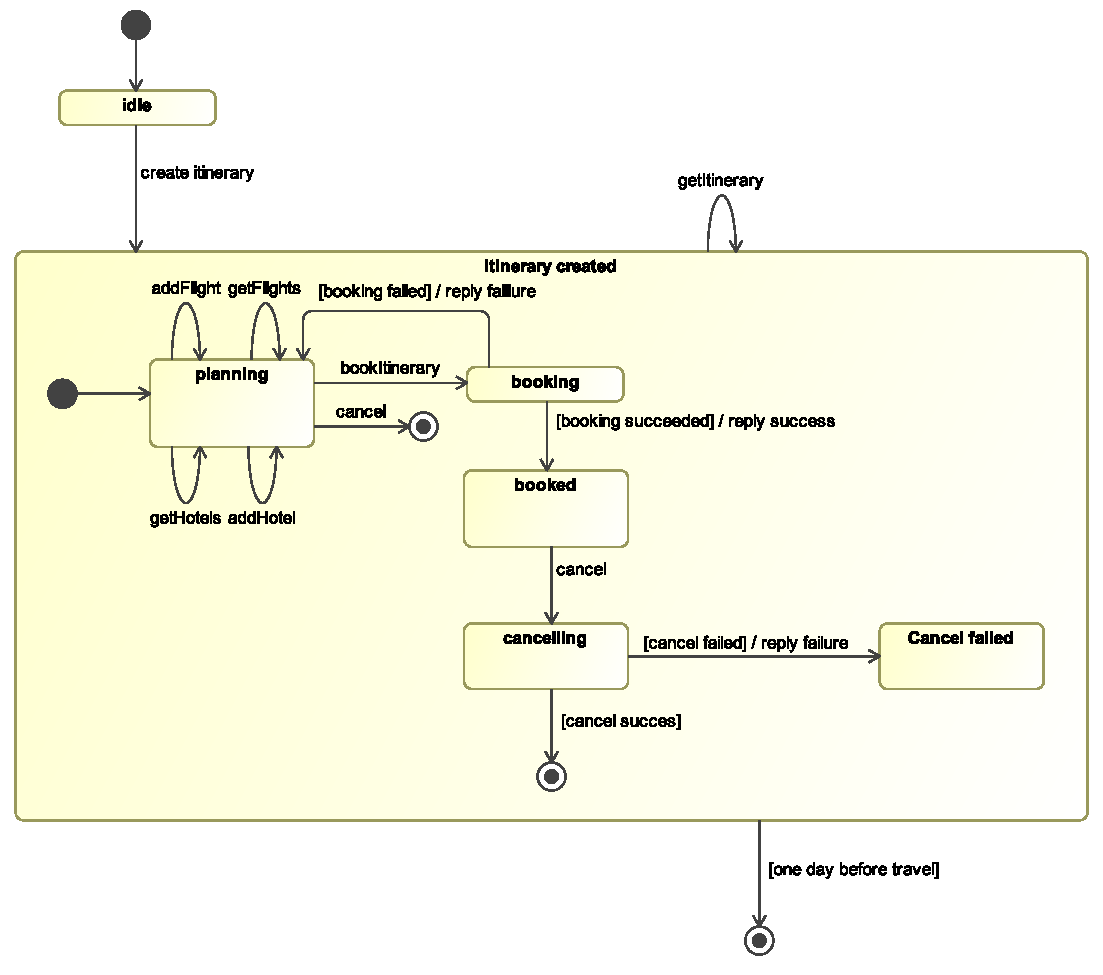
\includegraphics[width=1.0\textwidth]{Protocol}
\caption{Protocol for the TravelGood service, by \pet{}}
\label{fig:protocol}
\end{figure}

The protocol sits idle, until the client creates an itinerary. At this point we enter a planning state, where it is possible to search for flights and hotels, and add some of them to the itinerary. During this phase, the client is free to cancel planning and thus ending the protocol. If the client does not cancel, the itinerary can be booked, which will then be attempted. If the booking fails on any item in the itinerary, we return to the planning state and inform the client. 

Upon a successful booking the process continues to the booked state. From here, the client can try to cancel the booked flights and hotels and TravelGood will cancel as many items on the itinerary as possible. If all succeeds, we end the protocol -- otherwise we cancel as many as we can and go to a passive state. On the day before the travel starts, the protocol ends, if it is still running (i.e. is in the passive state). At any time during the protocol, the client can request the current itinerary.